\chapter{Entwurfsmuster}
\label{ch:Entwurfsmuster}

In diesem Kapitel soll exemplarisch die Verwendung von klassischen Entwurfsmustern gezeigt und begründet werden.
Außerdem wird die Verwendung der Entwurfsmuster jeweils mit einem UML-Klassendiagramm verdeutlicht.
\newline
Allgemein sind Entwurfsmuster wiederverwendbare und generalisierte Lösungen für häufige Problemstellungen.
Durch die Generalisierung müssen Entwurfsmuster teilweise für konkrete Anwendungsfälle angepasst werden, sodass die endgültige Lösung vom eigentlichen Entwurfsmuster abweichen kann.
Deshalb werden in den folgenden Abschnitten insbesondere auch die Abweichungen vom Muster in Reinform dokumentiert. 

\section{Composite}

Das \textbf{Composite} ist ein Strukturmuster, das es dem Verwender erlaubt, ein komplexes Objekt genauso zu verwenden wie ein einfaches Objekt.
Ein komplexes Objekt kann dabei aus einem oder mehreren Objekten bestehen, wobei ein solches Kind selbst wieder ein komplexes Objekt sein kann.
Im Gegensatz dazu besteht ein einfaches Objekt nicht aus mehreren Kindobjekten.
So können zum Beispiel auch Baumstrukturen abgebildet werden.
Der große Vorteil des Musters ist, dass der Verwender nicht unbedingt wissen muss, ob es sich um ein einfaches oder komplexes Objekt handelt
\cite[pp.~142--155]{geirhos2015entwurfsmuster}.
\newline
Das hier aufgeführte Anwendungsbeispiel umfasst das Interface \textit{ClientDataCallback} und die Klasse \textit{ClientDataCallbackComposite}, die das Interface implementiert.
Das Interface stellt eine Callback-Methode bereit, die ein Objekt vom Typ \textit{ResponseData} entgegennimmt.
Das ClientDataCallbackComposite wurde eingeführt, um es zu ermöglichen, mehrere Callback-Methoden mit einem Funktionsaufruf ausführen zu können.
Dies wird insbesondere benötigt, um die ResponseData-Objekte mit denen die Callback-Methoden aufgerufen werden im lokalen Cache ablegen zu können.
Die Funktionalität, ein Objekt in den Cache einzufügen wird demnach als einfache Callback-Methode übergeben und kann mit einer anderen Callback-Methode zusammen in einem Objekt gehalten werden.
\newline
Da das Composite-Muster dem Decorator-Muster strukturell sehr ähnlich ist, wurde die Klasse ClientDataCallbackDecorator auch erst mit Commit \href{https://github.com/lukaspanni/OpenSourceStats/commit/2198284a8f90a76a0e0a2e99f9be87855595458e}{2198284} in ClientDataCallbackComposite umbenannt, um klarer zu machen, was der Zweck dieser Klasse ist.
Ein Decorator wird eher dazu verwendet einem Objekt zur Laufzeit neues Verhalten hinzuzufügen, anstatt ein komplexes Objekt aus mehreren Einzelobjekten zusammenzusetzen \cite[pp.~155-169]{geirhos2015entwurfsmuster}.
Da der Zweck der Anwendung des Musters, gezeigt in Abbildung \ref{fig:pattern_composite}, ist, beliebig viele Callbacks mit nur einem Methodenaufruf ausführen zu können, wurde hier die Bezeichnung Composite gewählt.
Durch die sehr große strukturelle Ähnlichkeit der Muster könnte man in diesem einfachen Fall aber auch für die Benennung Decorator argumentieren.

\begin{figure}[h]
    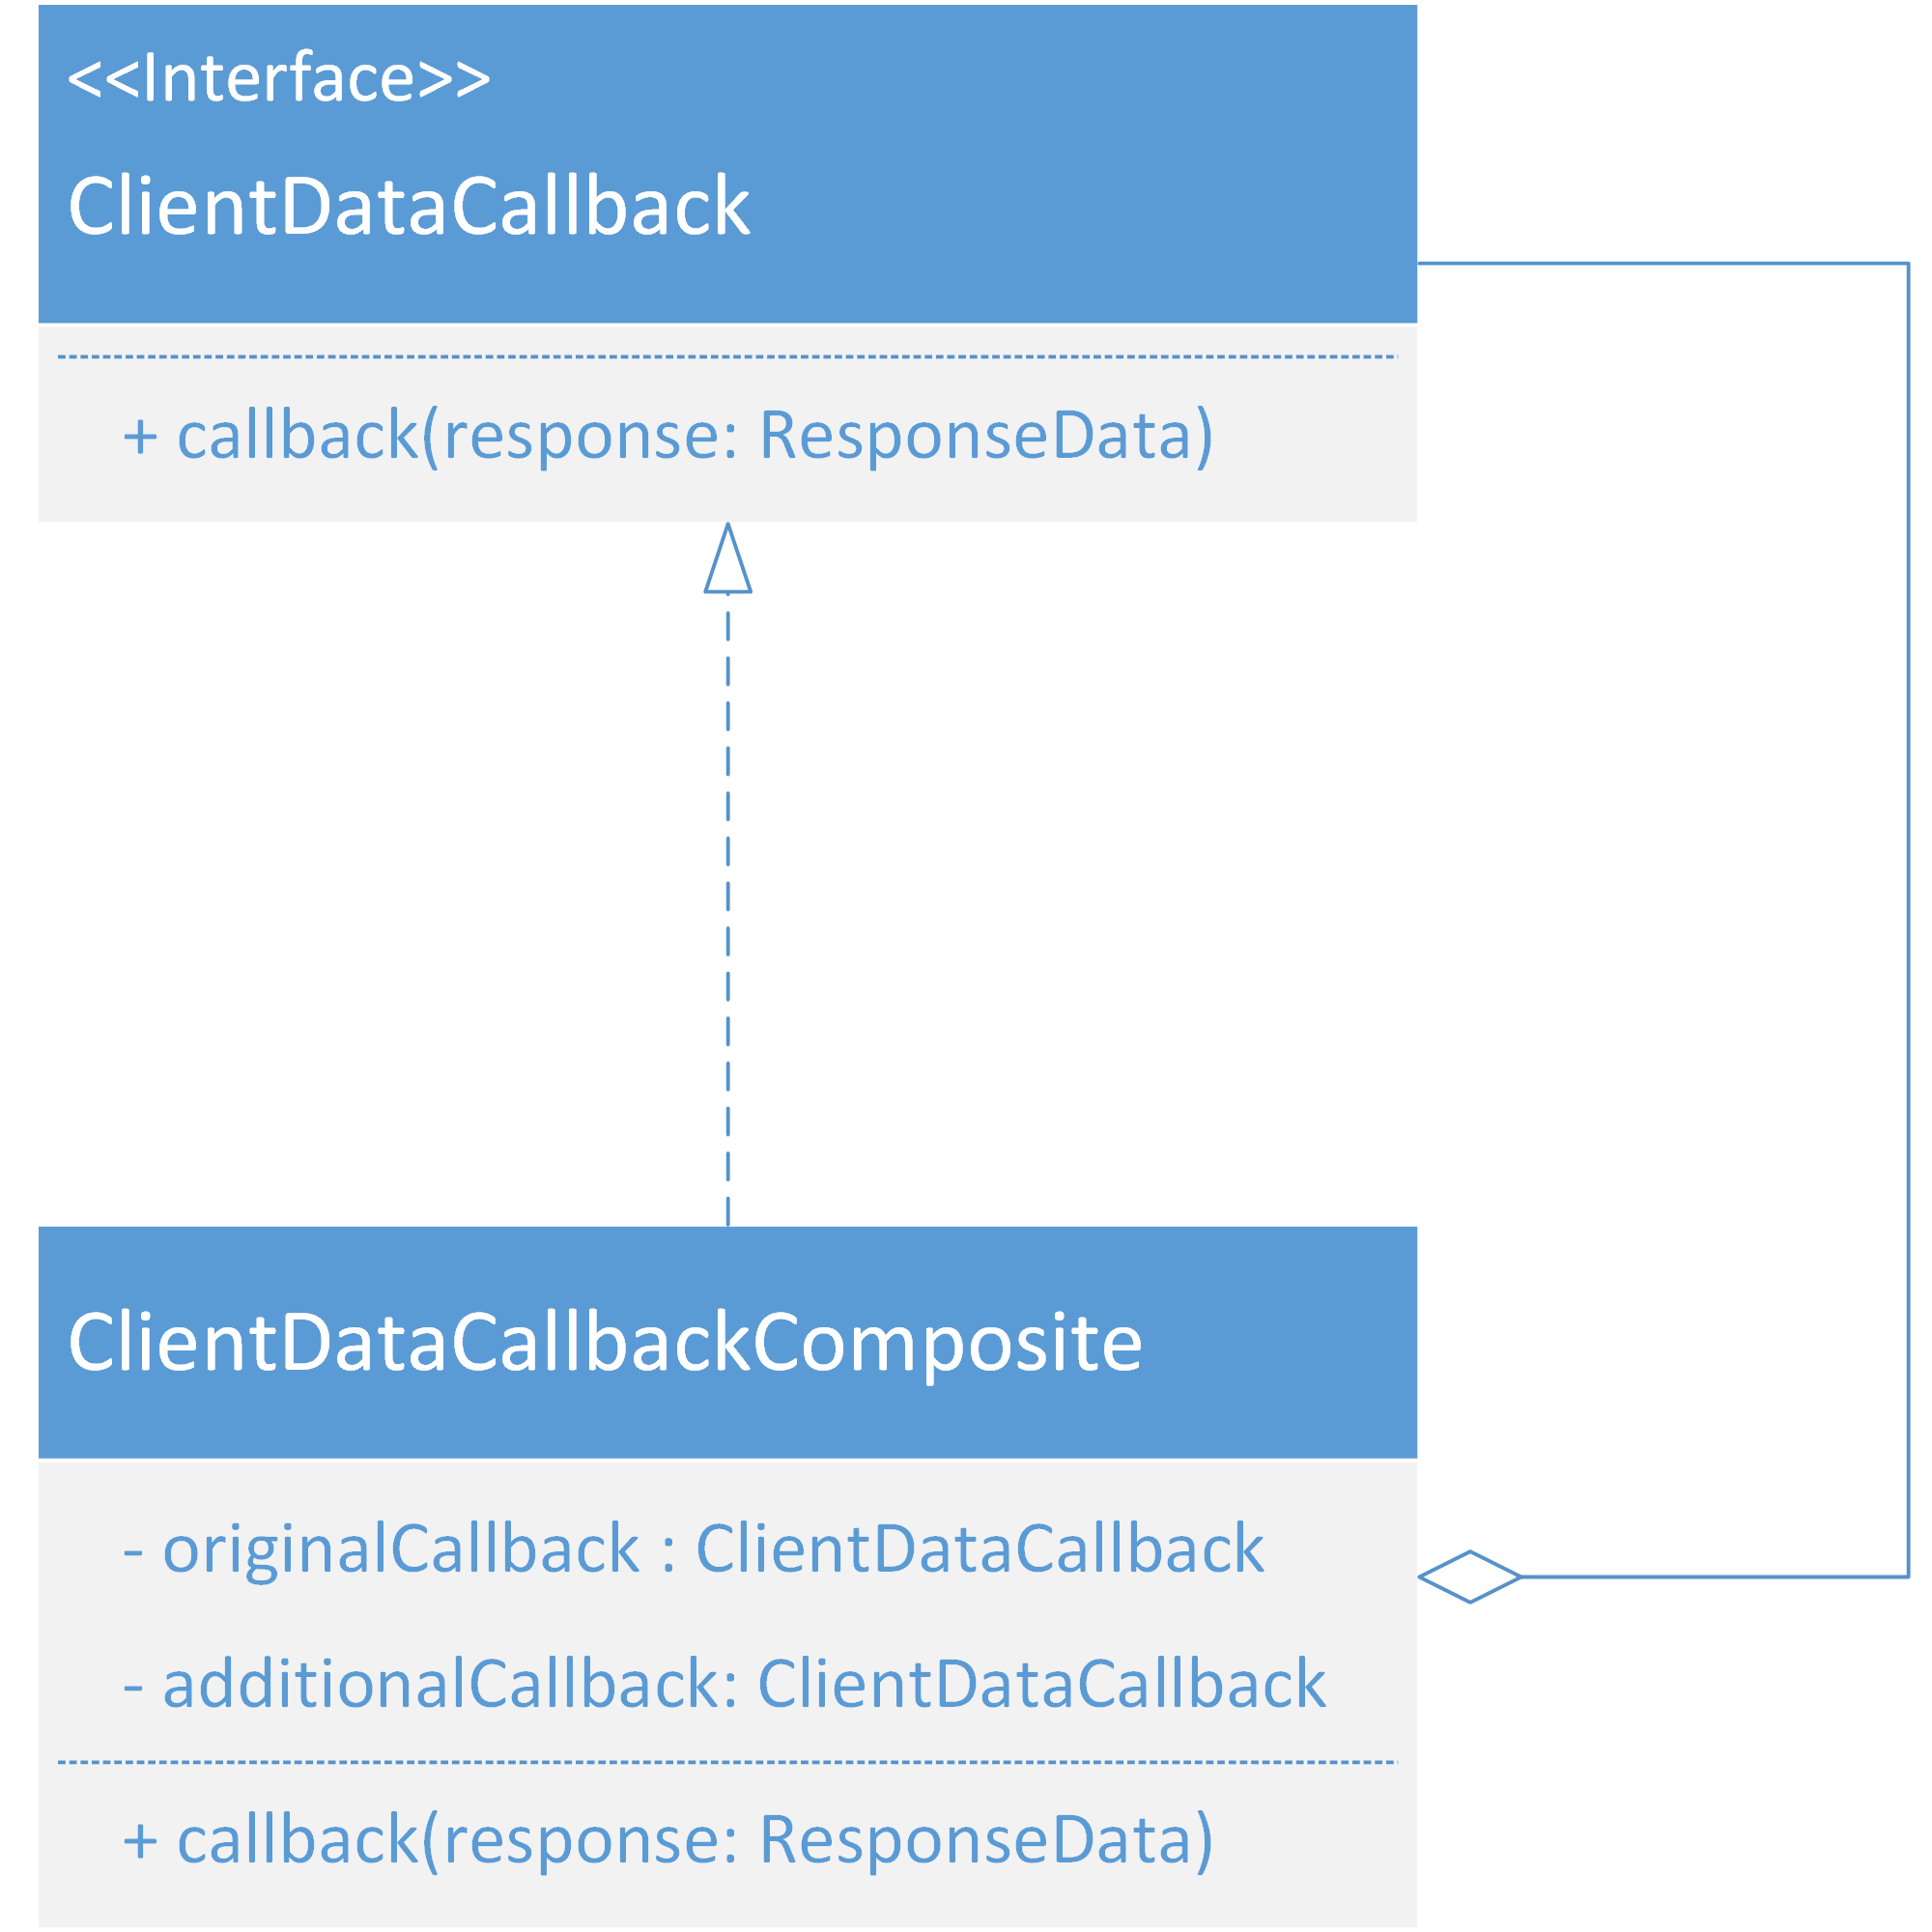
\includegraphics[scale=0.5]{pattern_composite.png}
    \centering
    \caption{Umsetzung des Composite Patterns}
    \label{fig:pattern_composite}
\end{figure}

\newpage
\section{Strategy}

\begin{figure}[h]
    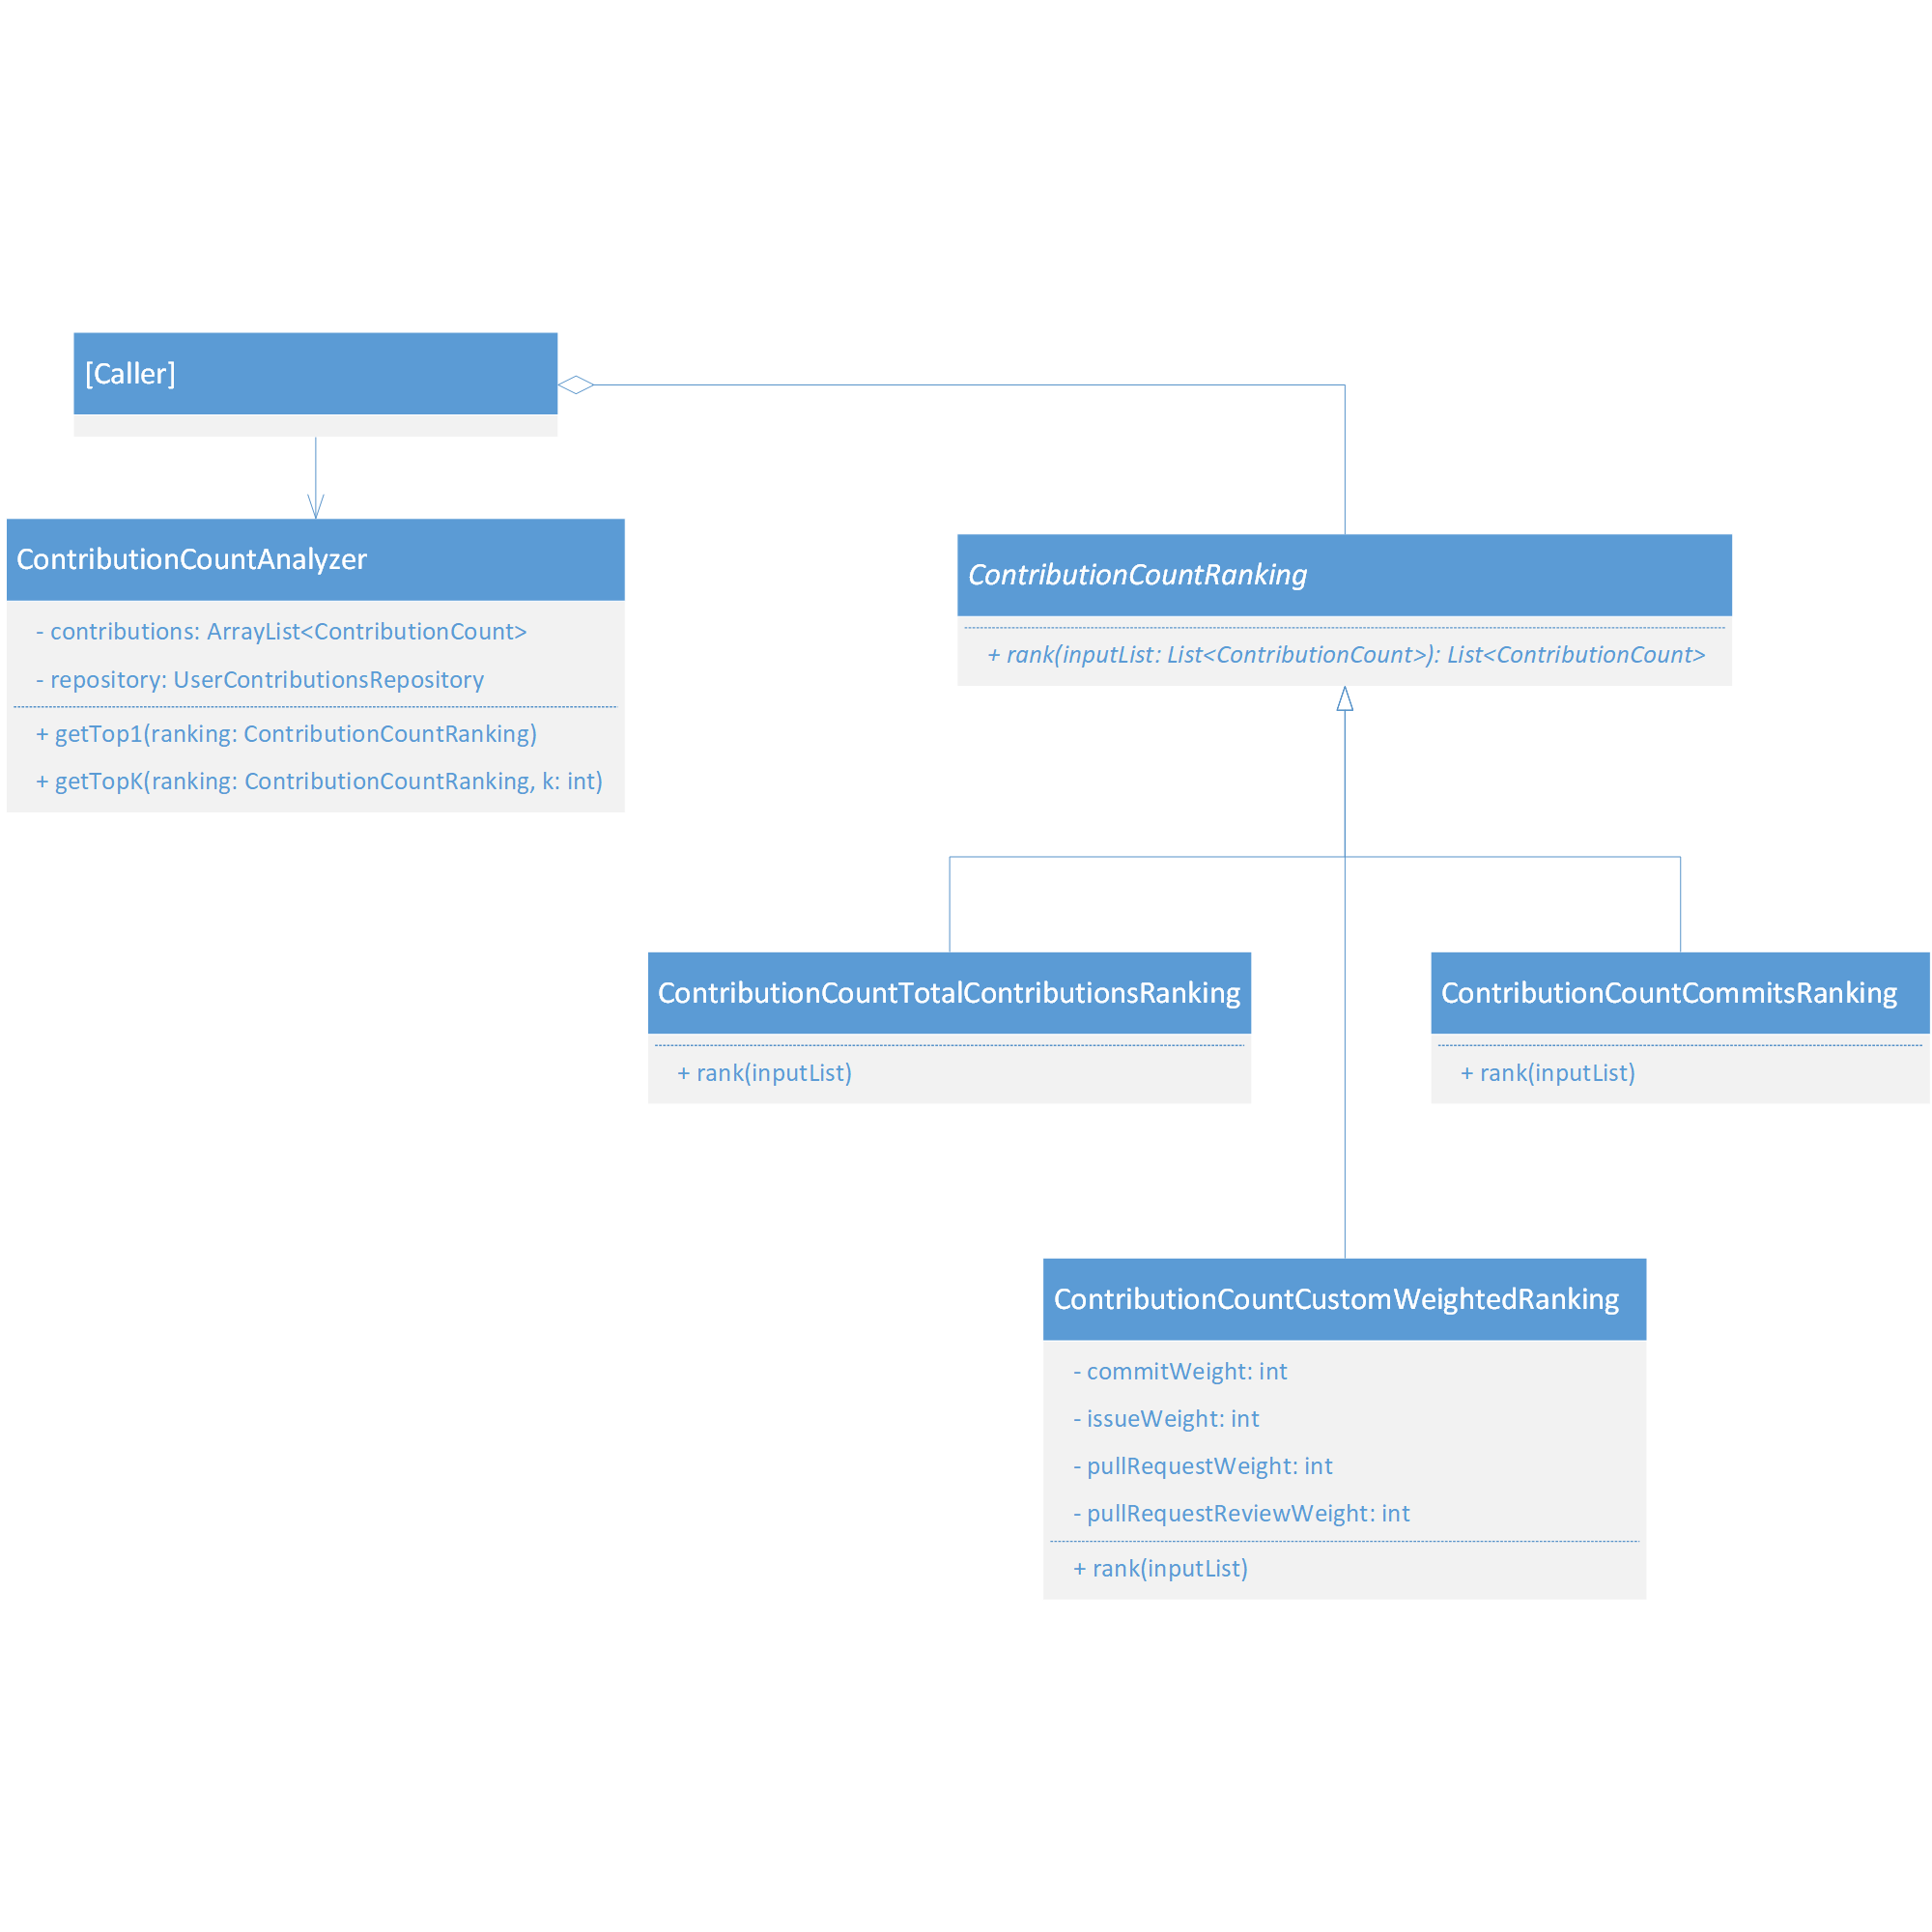
\includegraphics{pattern_strategy.png}
    \centering
    \caption{Umsetzung des Strategy-Patterns}
    \label{fig:pattern_strategy}
\end{figure}
